\section{RTOS}
\subsection{POSIX Threads Programming}
\subsubsection{UNIX Process}
\begin{itemize}
    \item Heavyweight process (created by the operating system)
    \item Each process has its own protected address space.
    \item Processses are isolated so that they cannot inadvertently infringe on each other.
    \item Because of this enforces separation, communications between processes can take place only by using OS kernel services.
    \item Processes require a fair amount of overhead; they contain information about program resources and program execution state, including: Process ID, process group ID, user ID, and group ID; Environment; Program instructions; Registers; Stack; Heap; File descriptors; Signal actions; Shared libraries; Inter-process communication tools
\end{itemize}

\subsubsection{UNIX Thread}
\begin{itemize}
    \item A POSIX thread is a single flow of execution that runs within a process.
    \item \textbf{Threads use and exist within the process resources}
    \item \textbf{A thread uses the same address space as other threads of the same process}
    \item The main thread can create additional threads if it is so programmed.
          Thus, a process is virtually a collection of one or more threads.
    \item Threads are able to be scheduled by the operating system
    \item Independent stream of instructions that may run simultaneously to other streams of instructions
    \item Procedure that runs independently from its main program
    \item A thread maintains its own: Stack pointer; Registers; Scheduling properties; Set of pending and blocked signals; Thread specific data
    \item Concurrent programs are usually achieved with threads
\end{itemize}

\subsubsection{Process vs. Thread in UNIX}
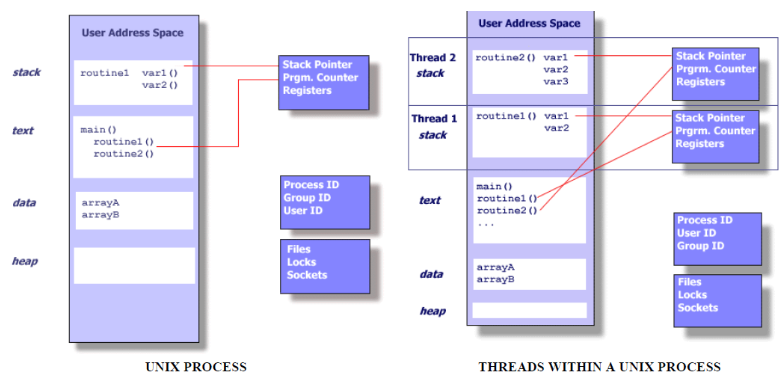
\includegraphics[width=12cm]{images/Concurrency/ProcessVsThread.png}

\subsection{What are POSIX Threads?}
\begin{itemize}
    \item For UNIX systems, a standardized C language threads programming interface has been specified by the \textbf{IEEE POSIX 1003.1c standard}.
    \item The short form of \textbf{POSIX threads} is \textbf{Pthreads} or \textbf{pthreads}.
    \item When compared to the cost of creating and managing a process, a thread can be created with much less operating system overhead
    \item Managing threads requires fewer system resources than managing processes
\end{itemize}

\subsection{Difference OS vs. RTOS}
A general purpose OS is system software that manages user applications and the hardware resources of a computer, defining rules and programming interfaces that allow a program to request OS services and interact with the rest of the system.
RTOS is an OS with many services commonly found in general-purpose OSs, such as multitasking, priority, task preemption, resource sharing, and intertask communication.
An RTOS is more than a general-purpose OS. An RTOS, with specialized scheduling algorithms, is intended to run real-time applications with soft and/or hard deadlines.
Thus, the key characteristic of an RTOS is that its response time to an event should be deterministic (or predictable).
An RTOS provides reliable mechanisms, such as real-time signals, preemptive scheduling, and nonblocking interprocess communications, for enabling a deterministic response.
\begin{itemize}
    \item RTOS is started in main
    \item Foreground and background process are dominating the OS
    \item A flow is a process or thread because the memory is not strictly isolated
    \item There are no sub flows
\end{itemize}
% \begin{paracol}{2}
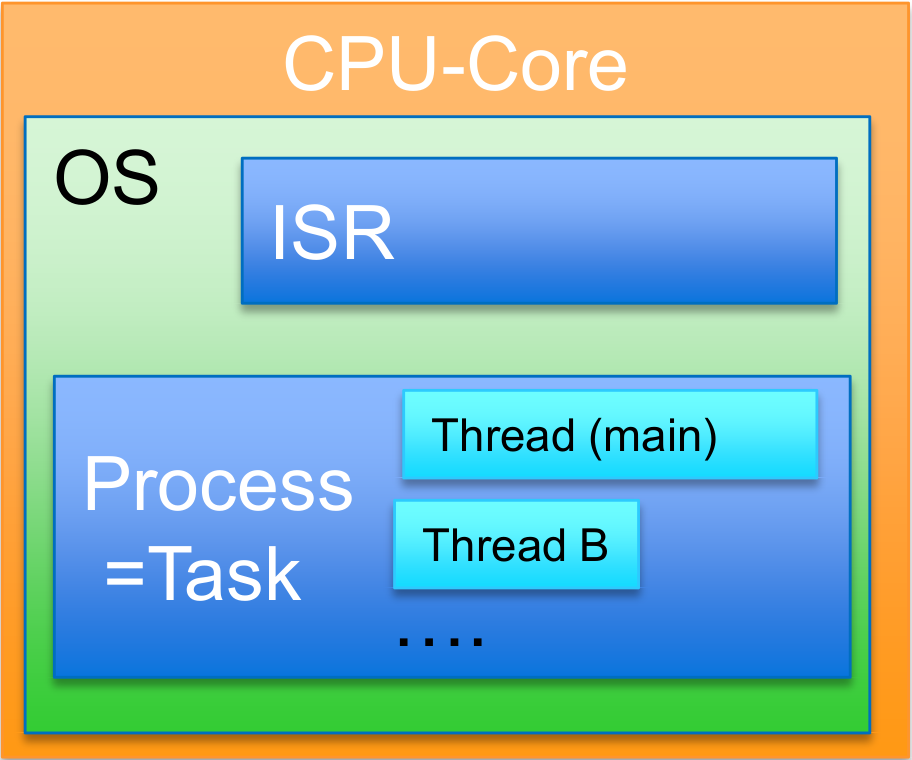
\includegraphics[width=0.25\textwidth]{images/Concurrency/os_process_thread.png}
% \switchcolumn
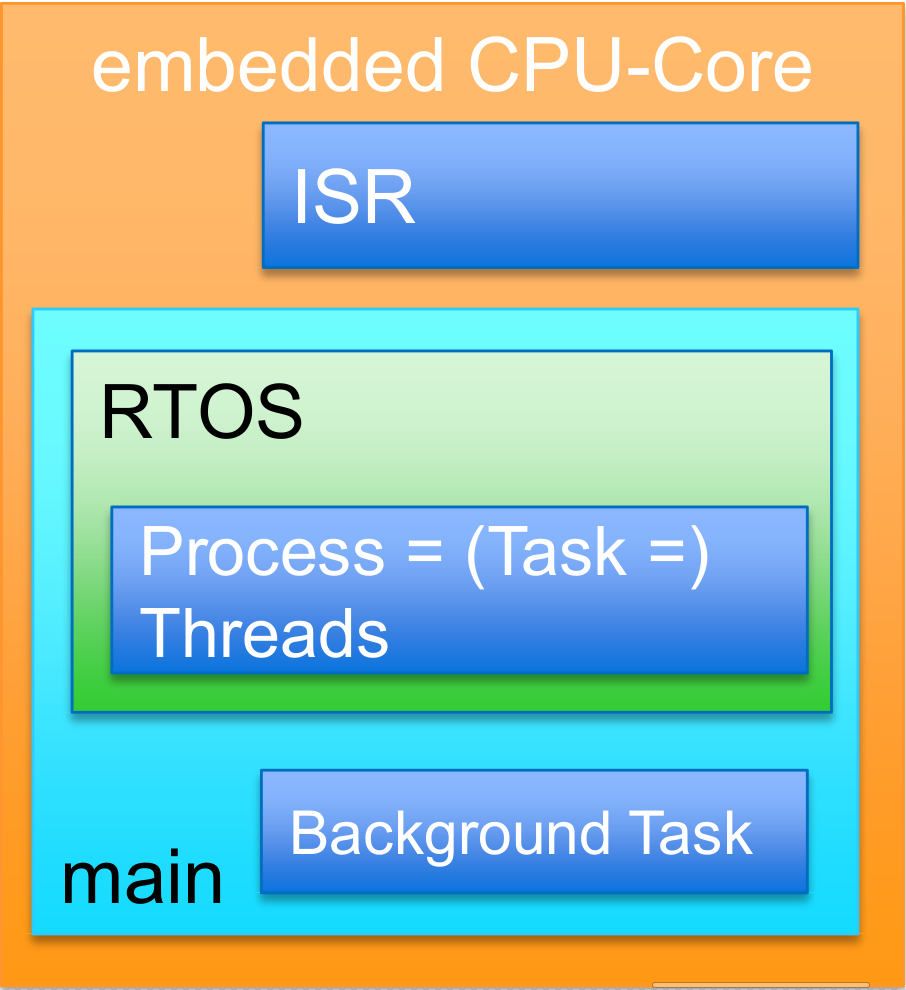
\includegraphics[width=0.25\textwidth]{images/Concurrency/rtos_process_thread.png}
% \end{paracol}

\subsection{System Structure}

\subsubsection{Scheduler and Dispatcher}
An RTOS needs at least one time basis.
This is often realized by one Timer with ISR!
The time basis defines how often a task can be dispatched.
This sets also some:
\begin{itemize}
    \item How high the overhead load for the CPU is
    \item Reaction time
    \item Timing constraints for WCE
\end{itemize}
The scheduler plans the next active Task according to priority and states of the task, which can be influenced by signals/events from ISR, main and tasks.\\
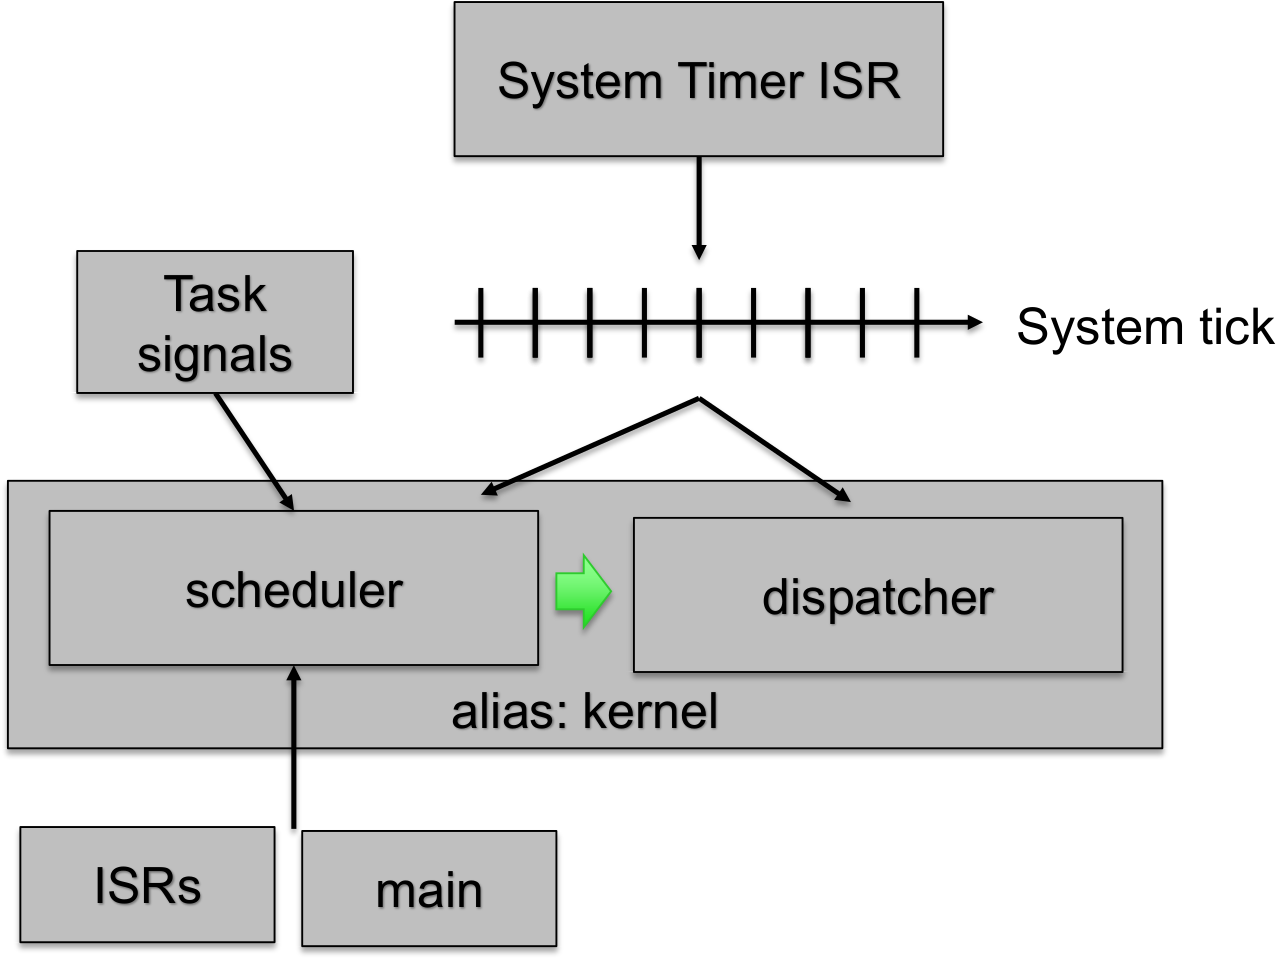
\includegraphics[width=0.5\textwidth]{images/RTOS/scheduler_dispatcher.png}

\subsubsection{Task States}
A task has different states, for instance:
\begin{itemize}
    \item Ready
    \item Running
    \item Blocked
    \item Sleeping
\end{itemize}
These terms are of the POSIX Standard, other RTOS may have different naming.\\
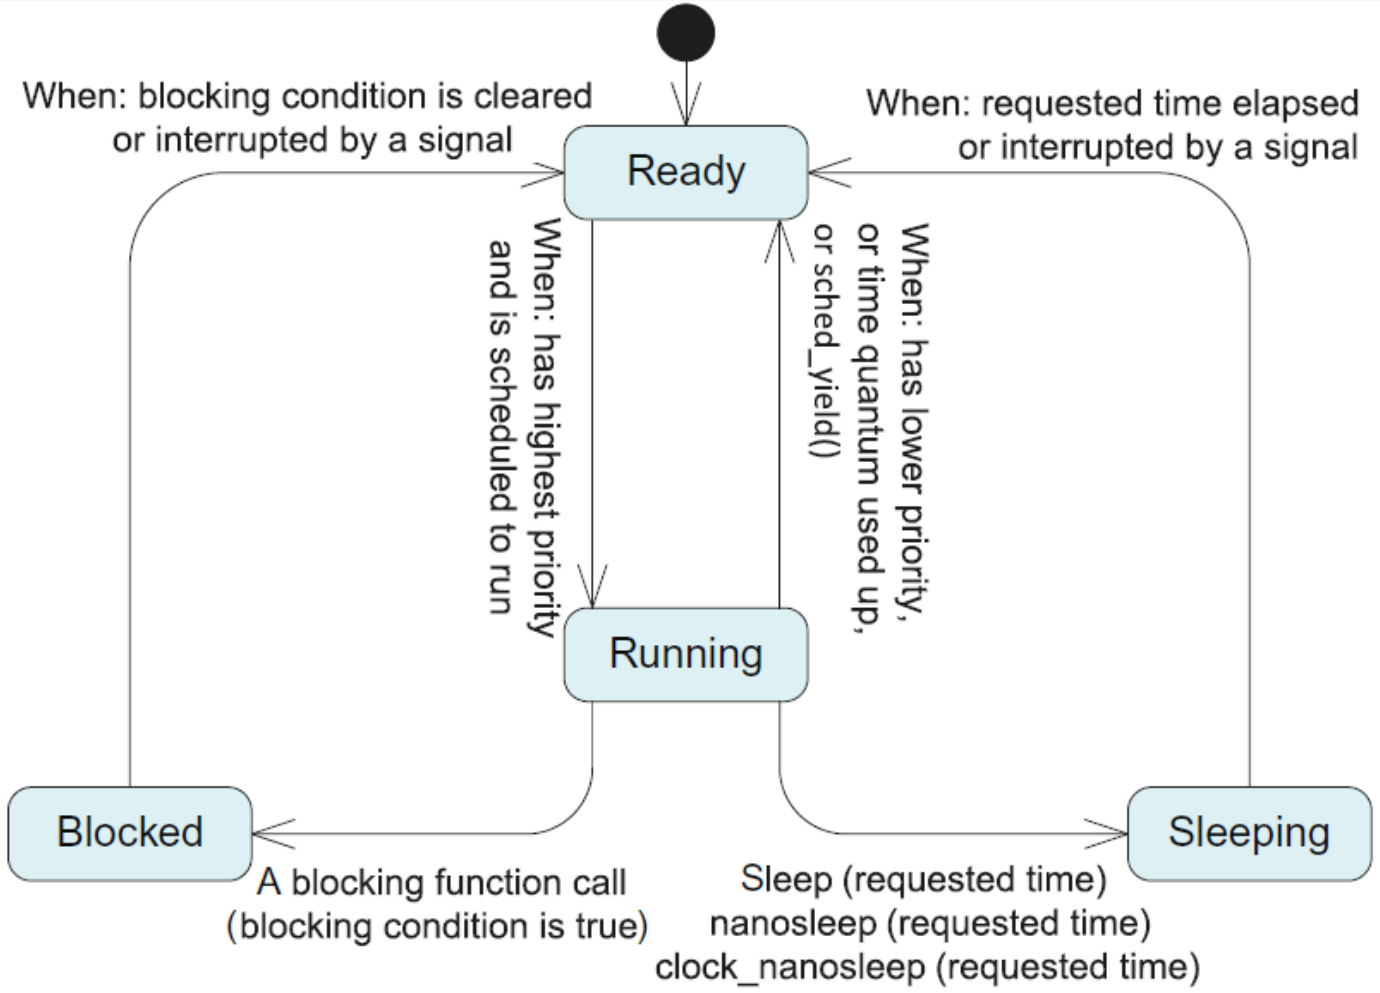
\includegraphics[width=0.5\textwidth]{images/RTOS/task_states_posix.png}
